\documentclass{report}
\usepackage[french,english]{babel}
\usepackage{geometry}
 \geometry{
 a4paper,
 total={150mm,245mm},
 left=30mm,
 top=25mm,
 }

\usepackage[nodayofweek,level]{datetime}
\usepackage[utf8]{inputenc}
\usepackage[T1]{fontenc}
\usepackage[toc,page]{appendix}
\usepackage{float}
\usepackage{import}
\usepackage{amsmath} 
\usepackage{graphicx}
\usepackage{caption}
\usepackage{subcaption}
\usepackage[usenames, dvipsnames]{color}
\usepackage{lipsum}
\usepackage{fancyhdr}

\graphicspath{ {images/} }

\begin{document}
\selectlanguage{english}
\pagenumbering{gobble}

\begin{titlepage}

\newcommand{\HRule}{\rule{\linewidth}{0.5mm}}
\center

\textsc{\LARGE LAMSADE}\\[1.5cm] 
\textsc{\Large M1 MIAGE}\\[0.5cm]
\textsc{\large Internship}\\[0.5cm] 

\HRule \\[0.4cm]
{ \huge \bfseries Internship Report} 
\HRule \\[1.5cm]

\begin{minipage}{0.4\textwidth}
\begin{flushleft} \large
\emph{Student:}\\
Elie \textsc{Abi Hanna Daher}\\ 
\textcolor{white}{blank space}
\end{flushleft}
\end{minipage}
~
\begin{minipage}{0.4\textwidth}
\begin{flushright} \large
\emph{Supervisor:} \\
M. Olivier \textsc{Cailloux} \\
M. Michel \textsc{Zam} 
\end{flushright}
\end{minipage}\\[2cm]

\newcommand{\mydate}{\formatdate{25}{8}{2017}}
{\large \mydate}\\[2cm] 

\begin{figure}[h]
\makebox[\textwidth]{

\includegraphics[width=0.40\textwidth]{dauphine.png}
\hfill    

\includegraphics[width=0.40\textwidth]{lamsade.png}
}\\[0.5cm]
\end{figure}

\vfill

\end{titlepage}

\abstract 
This report documents the work done during the summer internship at LAMSADE Dauphine, under the supervision of Mr. Olivier Cailloux and Mr. Michel Zam. The report give an overview of the projects completed during the internship.\\
I have worked mainly on the UTA method which is an ordinal regression method, proposed by E. Jacquete-Lagreze and J. Siskos, which adjust a system of additive utility function.\\
\tableofcontents{}
\pagenumbering{arabic}

\chapter{Introduction}
During my first year in Masters MIAGE at Paris Dauphine University, I had the opportunity to achieve an internship at LAMSADE (Laboratoire d'analyse et modélisation de systèmes pour l'aide à la décision). LAMSADE is a Paris-Dauphine research laboratory specialized in decision theoretic approaches. Decision theory aims at helping individuals who face decision problem by elaborating a study of the reasoning underlying agent's choices. \\

From \formatdate{29}{5}{2017} to \formatdate{1}{9}{2017}, I completed a research internship at LAMSADE at Paris Dauphine University. My internship was made remotely, so I had a meeting with Mr. Cailloux every week to get feedback of the work done. And I communicated with Mr. Zam via mails or calls. \\

This internship was very important for my professional career because it may be my last internship before I get my Masters's degree in Information systems for finance at Paris Dauphine University. Let's not also forget that this internship will allow me to practice the different courses learned during my academic years.\\

One of the objectives is to propose the UTA method as an open source software component. Another objective is to integrate this open source software into DecisionCloud, a software based on MyDraft a tool developed by KarmicSoft a LAMSADE spin-off. Researching similar literature and research represent an important objective in this internship. \\

In this report, I will present the context of the internship. It contains an overview of the projects realized: UTA, LinearProgramSolver, Research, DecisionCloud... Writing this report, I will also conclude by reflecting on my learning objects and goals achieved and not achieved.\\

\chapter{Context of the projects}

\chapter{Description of the projects}

\section{UTA}
\subsection{Introduction of the aid decision}
In decision theory a basic problem involving several criterias, concerns the way that the final decision should be made. However, this problem is posed in the opposite way: assuming that the decision is given, how is it possible to find the rational basis for the decision being made? Or how is it possible to assess the model leading to exactly the same decision as the actual one or the most "similar" decision.\\

In multicriteria decision aid methods (MCDA), the following concepts play a fundamental role in decision-making problems: 
\begin{enumerate}
\item object of the decision, definition of the set of potential actions(alternatives) and the determination of a problem statement
\item modeling a consistent family of criteria
\item defining a global preference model
\item decision-aid or decision support
\end{enumerate}

\underline{Example: Buying a new car} \\
Let's consider we are trying to figure out which car to buy. Using the methodology represented above, we state that the objective of this problem is \textbf{buying a new car}. After stating the objective, we can list the potential of actions that represent the list of cars that we may buy. By potential action, we designate that which constitutes the object of the decision. An action is qualifed as potential when it is deemed possible to implement it or if it has some interest within the decision aiding process. So the following list represent the potential actions of this example: 
\begin{itemize}
\item Peugeot 208 GTi
\item Nissan Sentra
\item Citroen C4
\item Peugeot 308 berline
\end{itemize}
After listing the list of potential cars, we can define a list of criteria that we will base our decision on. A criterion is contructed to evalute and compare potential actions according to a point of view. So when defining the list of criteria you should always remember that they must be easy to evaluate (easy to convert to a scale) and should be logical.
Let's say we will base our purchase on the following criteria:
\begin{itemize}
\item price (in Euro)
\item comfort (0, +, ++, +++) \textit{0 being not comfortable and +++ very comfortable}
\item safety (1, 2, 3, 4, 5) \textit{1 being not safety and 5 safe}
\end{itemize}
During the decision process, we will determinate the global preferences of the potential actions:
\begin{enumerate}
\item Citroen C4
\item Peugeot 208 GTi
\item Peugeot 308 berline
\item Nissan Sentra
\end{enumerate}
Once the global preference is defined, we can start the decision support.\\

One of the multi-criteria decision analysis methods is the UTA method, which was proposed by E. Jacquet-Lagrèze and J. Siskos in 1982. This method is proposed by the Multi-Attribute Utility Theory (MAUT) that build a utility function based on the DM\footnote{Decision Maker} preferences.\\
 
The UTA method is used to solve a multi-criteria problem by building a utility function based on the preferences of the DM and solving a linear program (LP). It adopt the aggregation-disaggregation principles: where the model is based on a given preferences.\\

The UTASTAR, a variant of the UTA method, has been considered a better algorithm than UTA. Better result were found using the UTASTAR algorithm. So this is why we will focus on this method rather than the UTA method.\\

The aim of the UTASTAR method is to estimate a set of additive utility functions which are as consistent as possible with the decision maker's preferences.\\

At the begining of the problem, the DM should present the following information 
\begin{itemize}
\item rank of the actions
\item give the criteria he want to base his decision on 
\item evaluate the action compared to the criterion
\end{itemize}
Once those information are presented, the UTASTAR algorithm can be executed. 

\newpage
\subsection{Principles and Notation}
Let's call $A={a,b,c,...}$ the set of potential actions and $g_1, g_2, g_3, ..., g_n$ the family of criteria. Where $g_i(a)$ represent the funtion of an action(alternative)$a$ on the criteria $g_i$ with $a \in A_R$. \\

We define $g_{i*}$ as the least preferred criteria: $g_{i*} = min_{a \in A} g_i (a)$ and $g_i^{*}$ as the most preferred criteria: $g_i^{*} = max_{a \in A} g_i (a)$. So the interval for each criteria $g_i$ is: $[g_{i*} , g_i^{*}]$.\\

If we want to evaluate two actions, for example $a$ and $b$, on only one criteria $g_i$ we have the following relations: 
\begin{equation}
      \begin{cases}
      	a \succ b\Leftrightarrow g_i(a) > g_i(b) \quad preference\\
      	a\sim b \Leftrightarrow g_i(a) = g_i(b) \quad indifference \\
      \end{cases}
\end{equation}
The criteria aggregation model in UTASTAR has the following form:
\begin{equation}\label{eq1}
      v(g(a)) = \sum_{i=1}^{n} v_i (g_i (a))
\end{equation}
subject to normalization constraints:\\
\begin{equation}\label{eq2}
      \begin{cases}
      	\sum_{i=1}^{n} v_i(g_{i}^{*}) = 1\\
       	v_i(g_{i*})= v_i(g_i^1)  = 0,  \forall i = 1, 2, ..., n\\
      \end{cases}
\end{equation}
where $ v_i, i = 1,2,...,n$ are non decreasing real valued function.\\

In UTASTAR we have 
\begin{equation}
	w_{ij} = v_i(g_i^{j+1}) - v_i(g_i^{j}) \geq 0 \quad \forall i \quad j 
\end{equation}

Which will allow us to write: 
\begin{equation}
	v_i(g_i^j) =	  \sum_{t=1}^{j-1} w_{it} \quad \forall i = 1,2,...,n \quad and \quad j = 2,3,...,\alpha _i -1 \\
\end{equation}

With the evaluation of an action a $g(a) = [g_1(a) ,  g_2(a) , ... , g_n(a)] $, we have the following relation:
\begin{equation}
      \begin{cases}
      	v[g(a)] > v[g(b)] \Leftrightarrow a \succ b\\
      	v[g(a)] \sim v[g(b)] \Leftrightarrow a = b\\
      \end{cases}
\end{equation}

\newpage
\subsection{Development} 
The updated version of UTA, UTASTAR, propose a double error function for each action: $\sigma ^{+} (a)$ and $\sigma ^{-} (a)$.  So the value of each alternative $a \in A_R$ can be written: \\
\begin{equation}
	v^{'} [g(a)] = \sum_{i=1}^{n} v_i [g_i (a)] - \sigma ^{+} (a)+ \sigma ^{-} (a) \quad  \forall a \in A_R
\end{equation}
\begin{figure}[H]
    	\centering
	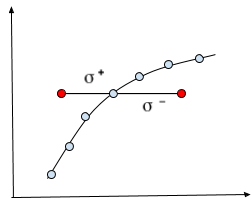
\includegraphics{error-function-utastar}
	\caption{Error function in UTASTAR}
\end{figure}
For each criteria, the interval $[g_{i*}, g_i^{*}]$ is cut into $(\alpha _i -1)$ equals interval, and the end points $g_i^{j}$ are given by the formula:
\begin{equation}
	g_i^{j}= g_{i*} + \frac{j-1}{\alpha _i -1} (g_i^{*} - g_{i*})  \forall j = 1,2, ..., \alpha _i
\end{equation}

The marginal value of an action $a$ is calculated by a linear interpolation
\begin{equation}
	v_i [g_i (a)] = v_i (g_i^{j}) + \frac{g_i (a) - g_i^{j}}{ g_i^{j+1} - g_i^{j}} [v_i (g_i^{j+1}) - v_i (g_i^{j}) ] 
\end{equation}

The set of reference action $ A_R = a_1, a_2, ... , a_m$ is arranged where $a_1$ is the best action and $a_m$ is the worst action. Which indicate that we have two possible situations:
\begin{itemize}
\item $a_k  \succ a_{k+1} \quad $ preference 
\item $a_k \sim a_{k+1} \quad $ indifference
\end{itemize} 

So if we have that $\Delta (a_k, a_{k+1} ) = v^{'} [g(a_k)] - v^{'} [g(a_{k+1})]$ and $\delta$ is a small positive number we will obtain the following relations: 
\begin{equation}\label{eq3}
      \begin{cases}
      	\Delta (a_k, a_{k+1} ) \geq \delta\\
       	\Delta (a_k, a_{k+1} ) = 0 \\
      \end{cases}
\end{equation}
The marginal value functions are estimated by means of the Linear Programm with \eqref{eq1}, \eqref{eq2}, \eqref{eq3} as constraints, and an objective function depending on the $ \sigma^{+}$ and $\sigma^{-} $: 
$$ [min]z = \sum_{k=1}^{m} [ \sigma ^{+} (a_k) + \sigma ^{-} (a_k)]  $$
subject to: 
\begin{equation}\label{eq5}
      \begin{cases}
      	\Delta (a_k, a_{k+1} ) \geq \delta \quad or \quad \Delta (a_k, a_{k+1} ) = 0 \\
      	\sum_{i=1}^{n} \sum_{j=1}^{\alpha_i -1} w_{ij} = 1\\
       	w_{ij} \geq 0, \quad \sigma^{+}(a_k) \geq 0, \quad \sigma^{-}(a_k) \geq 0, \quad  \forall i, j  and  k\\
      \end{cases}
\end{equation}

\subsection{Example}
The implementation of UTASTAR algorithm is illustrated by the example from the Introduction chapter : \textbf{buying a new car}.\\ The DM is interested only in the following criteria:
\begin{itemize}
\item price (in Euro)
\item comfort ($0$, +, ++, +++) \textit{0 being not comfortable and +++ very comfortable}
\item safety ($1, 2, 3, 4, 5$) \textit{1 being not safety and 5 safe}
\end{itemize}
The evaluation of the previous criteria is presented in the following table: 
\begin{center}
 \begin{tabular}{|c | c c c c|} 
 \hline
 Cars & Price & Comfort & Safety & Ranking of the DM \\ [0.5ex] 
 \hline
 Nissan Sentra (ns) & 17\,000 & +++ & 4 & 1 \\ 
 \hline
 Citroen C4 (c4) & 15\,000& ++ & 2 & 2\\ 
 \hline
 Peugeot 208 GT (p208) & 25\,000 & + & 3 & 3\\
 \hline
 Peugeot 308 berline (p308)& 18\,500 & 0 & 3 & 4\\
 \hline
\end{tabular}
\end{center}
First of all, we should specify the scale \footnote{the interval $[g_{i*}, g_{i}^{*}]$ is cut into equal intervals} for each criteria.
\begin{itemize}
\item Price $\quad \Rightarrow \quad [g_{1*}, g_{1}^{*}] = [25\,000, 20\,000, 15\,000]$
\item Comfort $\quad \Rightarrow \quad [g_{2*}, g_{2}^{*}] = [0, +, ++, +++]$
\item Safety $\quad \Rightarrow \quad [g_{3*}, g_{3}^{*}] = [1, 3, 5]$
\end{itemize}
According to this formula: $v(g(a)) = \sum_{i=1}^{n} v_i (g_i (a))$ , the value of each alternative may be written: 
\begin{itemize}
\item $v(g(ns)) =  0.4v_1(15\,000) +  0.6v_1(20\,000) + v_2(+++) + 0.5v_3(3) + 0.5v_3(5)  $
\item $v(g(c4)) = v_1(15\,000) + v_2(++) + 0.5 v_3(1) + 0.5v_3(3) = v_1(15\,000) + v_2(++) + 0.5v_3(3)$
\item $v(g(p208)) = v_1(25\,000) + v_2(+) + v_3(3) = v_2(+) + v_3(3) $
\item $v(g(p308)) = 0.3v_1(15\,000) +  0.7v_1(20\,000) + v_2(0) + v_3(3) = 0.3v_1(15\,000) +  0.7v_1(20\,000) + v_3(3)$
\end{itemize}
We have that $v_1(25\,000) = v_2(0) = v_3(1) = 0$. \\
Since the marginal value $u_i(g_i)$ can be expressed in terms of variables $w_{ij}$: $u_i(g_i^{j}) = \sum _{t=1}^{j-1} w_{it}$ , the value of each alternatie can be written: 
\begin{itemize}
\item $v(g(ns)) = w_{11} + 0.4w_{12} + w_{21} + w_{22} + w_{23} + w_{31} + 0.5w_{32}$
\item $v(g(c4)) = w_{11} + w_{12} + w_{21} + w_{22} + 0.5w_{31}$
\item $v(g(p208)) = w_{21} + w_{31} $
\item $v(g(p308)) = w_{11} + 0.3w_{12} + w_{31}$
\end{itemize}
For each pair of consecutive alternatives, we express the difference between them: 
\begin{itemize}
\item $\Delta (ns,c4) =  -0.6w_{12} + w_{23} + 0.5w_{31} +  0.5w_{32}  -\sigma _{ns}^{+} +\sigma _{ns}^{-} +\sigma _{c4}^{+} - \sigma _{c4}^{-} $
\item $\Delta (c4, p208) = w_{11} + w_{12} + w_{22} - 0.5w_{31} -\sigma _{c4}^{+} +\sigma _{c4}^{-} +\sigma _{p208}^{+} - \sigma _{p208}^{-} $
\item $\Delta (p208, p308) =w_{21} - w_{11} - 0.3w_{12} -\sigma _{p208}^{+} +\sigma _{p208}^{-} +\sigma _{p308}^{+} - \sigma _{p308}^{-} $
\end{itemize}
Having $\delta = 0.05$, we can solve the following LP:\\

Objective:  
\begin{equation}
	Minimize \quad \sum_{a \in A} \sigma _{a}^{+} + \sigma _{a}^{-}
\end{equation}

Subject to: \\
\begin{equation}
	\begin{cases}
		 -0.6w_{12} + w_{23} + 0.5w_{31} + 0.5w_{32}  -\sigma _{ns}^{+} +\sigma _{ns}^{-} +\sigma _{c4}^{+} - \sigma _{c4}^{-}   \geq 0.05\\
		w_{21} - w_{11} - 0.3w_{12} -\sigma _{p208}^{+} +\sigma _{p208}^{-} +\sigma _{p308}^{+} - \sigma _{p308}^{-}  \geq 0.05 \\
		- 0.1w_{12} - w_{21} - w_{22} - w_{23} - 0.5w_{32} -\sigma _{p308}^{+} +\sigma _{p308}^{-} +\sigma _{ns}^{+} - \sigma _{ns}^{-}  \geq 0.05 \\
		w_{11} + w_{12} + w_{21} + w_{22} + w_{23} + w_{31} + w_{32} = 1
	\end{cases}
\end{equation}
An optimal solution is $w_{12} = 0.34$, $w_{21} = 0.152$, $w_{31} = 0.51$ with $\sum_{a \in A} \sigma _{a}^{+} + \sigma _{a}^{-} = 0$. The utilities found for each alternative are as follows: \\ 
\begin{itemize}
\item $v(g(ns)) = 0.798$
\item $v(g(c4)) = 0.747$
\item $v(g(p208)) = 0.662 $
\item $v(g(p308)) = 0.62 $
\end{itemize}
Those utilities are consistent with the DM's preference ranking. 

The UTA method build a utility function based on the preferences of the DM and it consist in solving a linear program (LP) to solve a multi-criteria problem.\\

This method will elaborate a model of preferences which is as similiar as possible to the DM's preferences.\\

An improved version of the UTA is the UTASTAR. In UTA we used a single error $\sigma(a)$ in UTASTAR we use a double positive error function. The updated version has performed better than the regular method.

\section{Linear Program Solver}
One of the steps of the UTA algorithm is solving the Linear Program. So we can complete the UTA algorithm, I created an independant java application that has the objectif of solving the LP by finding the optimal solution.\\
So i can achieve this goal I had to use the google ortools (Optimization tools) library. You can find those library in the github repository under src/libs.
\begin{figure}[H]
    	\centering
	
\includegraphics[width=4cm,height=1.5cm,keepaspectratio]{lp-libs.png}
	\caption{Library used in the solver}
\end{figure}
Let's talk the following example:\\

Objective:  
\begin{equation}
Maximize \quad 10x_1 + 6x_2 + 4x_3
\end{equation}

subject to: \\
\begin{equation}
	\begin{cases}
		x_1 + x_2 + x_3 \leq 100\\
		10x_1 + 4x_2 + 5x_3 \leq 600\\
		2x_1 + 2x_2 + 6x_3 \leq 300\\
	\end{cases}
\end{equation}
So we can solve the LP, we need to create an instance of the solver:
\begin{figure}[H]
    	\centering
	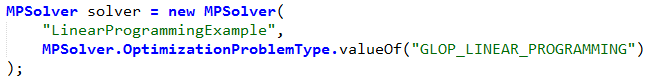
\includegraphics[width=\textwidth]{lp-solver.png}
	\caption{Java code to define the solver}
\end{figure}
After that, we define the 3 variables $x_1$, $x_2$ et $x_3 \quad  \in \quad [0 ; \infty]$: \\
\begin{figure}[H]
    	\centering
	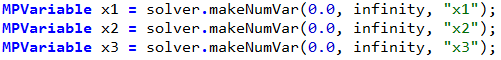
\includegraphics[width=10cm,height=3cm,keepaspectratio]{lp-variables.png}
	\caption{Java code to define the variables of the LP}
\end{figure}
We define the objective $Maximize \quad 10x_1 + 6x_2 + 4x_3$: \\
\begin{figure}[H]
    	\centering
	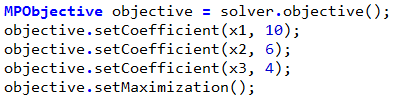
\includegraphics[width=8cm,height=2cm,keepaspectratio]{lp-objectif.png}
	\caption{Java code to define the objective of LP}
\end{figure}
We do the same for the constraint: \\
\begin{figure}[H]
    	\centering
	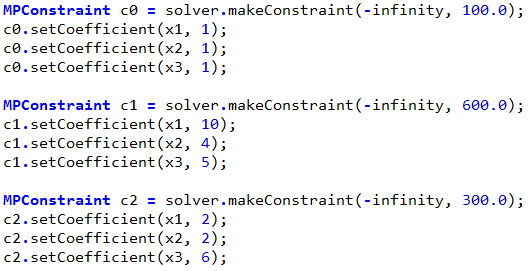
\includegraphics[width=10cm,height=6cm,keepaspectratio]{lp-constraints.png}
	\caption{Java code to define the constraints of the LP}
\end{figure}
After setting all the constraints and variables we can execute the solver: \\
\begin{figure}[H]
    	\centering
	
\includegraphics[width=10cm,height=6cm,keepaspectratio]{lp-solve.png}
	\caption{Java code for running the solver}
\end{figure}
After executing the solver, we display the optimal value of the objective and the value of the variables: \\
\begin{figure}[H]
    	\centering
	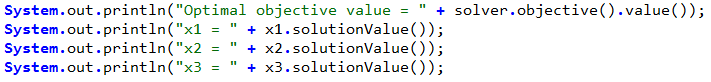
\includegraphics[width=\textwidth]{lp-result.png}
	\caption{Java code for displaying the result of the solver}
\end{figure}
Once you run the program, you will have the following the result: 
\begin{center}
Optimal objective value = 733.3333333333\\
x1 = 33.33333333336\\
x2 = 66.66666666666\\
x3 = 0.0\\
\end{center}

\section{Research}
A method of multicriteria analysis is chosen depending on the circumstances of the decision making.\\
UTA makes possible the estimation of a nonlinear additive function, which is obtained by the use of a linear program and the only information required from the decision maker are the global preferences between projects. \\
The value $\delta$ must not be given too high an initial value. \\
After the execution of the algorithm we should always be possible to converse with the decision maker in order to specify the precision of the preferences stated\\
In the basic model, it was noted that the values given to $\delta$ were to some extent arbitrary. UTAMP1 maximize $\delta$.\\
Variants of UTA\\
\begin{enumerate}
\item UTA
\item UTASTAR
\item UTA2
\item UTAMKEN
\item UTAMP1
\item UTAMP2
\item UTAMIME
\item UTASTARMIME
\item UTA2MIME
\end{enumerate}

Should i make a comparison table ??\\

Disadvantages\\
\begin{enumerate}
\item We can always question the decision marker about his preferences
\item Solution may not be the only one as in any LP we can have different solutions
\end{enumerate}


\chapter{Conclusion}

\begin{thebibliography}{9}
\addcontentsline{toc}{chapter}{Bibliography}
\bibitem{multiple-criteria-decision-analysis} GRECO S., EHRGOTT M., RUI FIGUEIRA J., 2004, \textit{Multiple Criteria Decision Analysis}
\bibitem{cahier-lamsade-24} SISKOS J., 1979, \textit{Cahier du LAMSADE n24 : Les programmes UTA}
\bibitem{cahier-lamsade-49} SISKOS J., YANNACOPOULOS D., 1982, \textit{Cahier du LAMSADE n49 : Amélioration de la méthode UTA par introduction d’une double fonction d’erreurs}
\bibitem{these-hammami} HAMMAMI A., 2003, \textit{Thèse : Modélisation technico-économique d’une chaîne logistique dans une entreprise reseau}
\bibitem{study-stock-ranking} LUO H., SUN Z., 2014, \textit{A study on Stock Ranking and Selection Strategy Based on UTA Method under the Condition of Inconsistence}
\bibitem{multicriteria-decision-aid-methodology} ZOPOUNIDIS C., DOUMPOS M., 1997, \textit{A multicriteria decision aid methodology for the assessment of country risk}
\bibitem{development-utastar-method-fuzzy} EHSANIFAR M., ESHLAGHI A., KERAMATI M., NAZEMI J., 2013, \textit{The Development of UTASTAR Method in Fuzzy Environment for Supplier Selection}
\bibitem{application-methode-uta} SISKOS J., 1983, \textit{Application de la méthode UTA à un problème de sélection de points de vente mettant en jeu des critères multiples}
\end{thebibliography}

\listoffigures
\addcontentsline{toc}{chapter}{Table of figures}

\begin{appendices}

\selectlanguage{french}
\chapter{Compte Rendus avec M. Cailloux}
\section{CR1 - 15 juin 2017}
\textbf{15 juin 2017} / 15:00 / Université Paris Dauphine \\

\underline{Participants} \\

Olivier Cailloux, Elie Daher\\

\underline{Déroulement de la réunion}\\
\begin{itemize}
	\item Explication du plan du stage
	\item J’ai présenté les tâches effectuées
	\item J’avais quelques questions sur la méthode UTA et plus précisément sur un exemple “A Numerical Example” du chapitre 9 : ”UTA Method” du livre : “Multiple Criteria Decision Analysis”
	\item Présentation des tâches à effectuer\\
\end{itemize}

\underline{Les tâches à faire} \\
\begin{itemize}
	\item Créer un repository sur github
	\item Ecrire un résumé sur la méthode UTA en utilisant LaTeX
	\item En parallèle, effectuer des recherches sur des littératures existantes\\
\end{itemize}

\underline{Pièces jointes} \\
\begin{itemize}
	\item First iteration : document présenté par M. Cailloux qui contient le plan de la première itération\\
\end{itemize}

La réunion a été levée à 15:30\\

La prochaine réunion est prévue pour le mercredi 21 juin 2017 à 14:00


\newpage
\section{CR2 - 21 juin 2017}
\textbf{21 juin 2017} / 14:00 / Université Paris Dauphine \\

\underline{Participants} \\

Olivier Cailloux, Elie Daher\\

\underline{Déroulement de la réunion} \\
\begin{itemize}
	\item Présentation du travail effectué
	\item Résolution du projet java sur le programme linéaire\\
\end{itemize}

\underline{Les tâches à faire} \\
\begin{itemize}
	\item Rendre le document plus détaillé et développé
	\item Rendre le document plus compréhensible pour les lecteurs qui n’ont pas un context décisionnel
	\item Fixer le programme linear programming sur Java\\
\end{itemize}

La réunion a été levée à 14:40\\

La prochaine réunion est prévue pour le mercredi 28 juin 2017 à 11:00
\newpage
\section{CR3 - 28 juin 2017}
\textbf{28 juin 2017} / 11:00 / Université Paris Dauphine \\

\underline{Participants} \\

Olivier Cailloux, Elie Daher\\

\underline{Déroulement de la réunion}\\
\begin{itemize}
	\item Présentation du travail effectué
	\item Citer les remarques et les modifications à réaliser sur le document summary-uta et sur le repository de github (enlever le folder qui contient les *.class)
	\item Présentation du travail à effectuer pour la semaine prochaine\\
\end{itemize}

\underline{Les tâches à faire} \\
\begin{itemize}
	\item Corriger les remarques sur le document
	\item Développer $v^R$ et $v^T$
	\item Effectuer une recherche sur les littératures similaires déjà réalisées\\
\end{itemize}

La réunion a été levée à 11:30\\

La prochaine réunion est prévue pour le mercredi 5 juillet 2017 à 10:00

\newpage
\section{CR4 - 18 juillet 2017}
\textbf{18 juillet 2017} / 10:00 / Université Paris Dauphine \\

\underline{Participants} \\

Olivier Cailloux, Elie Daher\\

\underline{Déroulement de la réunion}\\
\begin{itemize}
	\item Présentation du travail effectué
	\item Explication de la fusion entre le projet Alternative-Criteria et UTA
	\item Apprendre comment télécharger des littératures à partir du site de la BU de Dauphine\\
\end{itemize}

\underline{Les tâches à faire} \\
\begin{itemize}
	\item Elaborer un document qui regroupe tout le travail effectué
	\item S’approfondir dans la recherche des littératures
	\item Fixer la méthode GenerateNumbers\\
\end{itemize}

La réunion a été levée à 10:45\\

La prochaine réunion est prévue pour le mardi 25 juillet 2017 à 10:00

\newpage
\section{CR5 - 25 juillet 2017}
\textbf{25 juillet 2017} / 10:00 / Université Paris Dauphine \\

\underline{Participants} \\

Olivier Cailloux, Elie Daher\\

\underline{Déroulement de la réunion}\\

\underline{Les tâches à faire} \\

La réunion a été levée à \\

La prochaine réunion est prévue pour le 2017 à 

\chapter{Example of UTASTAR - Analyzing the choice of transportation}
A DM wants to analyse the choice of transportation. The DM is interstered in the following criteria 
\begin{enumerate}
\item price
\item time (min)
\item comfort (possibility to have a seat)
\end{enumerate}\leavevmode
The evaluation of the previous criteria is presented in the following table: 
\begin{center}
\begin{tabular}{ |c|c|c|c|c| } 
\hline
Means of transportation & Price & Time & Comfort & Ranking of the DM \\
\hline
RER & 3 & 10 & + & 1 \\
METRO (1) & 4 & 20 & ++ & 2 \\
METRO (2) & 2 & 20 & 0 & 2 \\
BUS & 6 & 40 & 0 & 3 \\
TAXI & 30 & 30 & +++ & 4 \\
\hline
\end{tabular}
\end{center}
DM's preferences: $ RER \succ  Metro1 \approx Metro2  \succ  Bus \succ  Taxi$\\
\newpage
First of all, we should specify the scale \footnote{the interval $[g_{i*}, g_{i}^{*}]$ is cut into equal intervals} for each criteria.
\begin{itemize}
\item Price  $\quad \rightarrow \quad [30, 16, 2]$
\item Time  $\quad \rightarrow \quad [40, 30, 20, 10]$
\item Comfort  $\quad \rightarrow \quad [0, +, ++, +++]$
\end{itemize}
According to this formula: $v(g(a)) = \sum_{i=1}^{n} v_i (g_i (a))$ , the value of each alternative may be written: 
\begin{itemize}
\item $v[g(RER)]= 0.07  v_1 (16) + 0.93 v_1(2) + v_2(10) + v_3(+)$
\item $v[g(METRO1)]= 0.14 v_1 (16) + 0.86 v_1(2) + v_2(20) + v_3(++)$
\item $v[g(METRO2)]= v_1 (2) + v_2(20) + v_3(0) =  v_1 (2) + v_2(20) $
\item $v[g(BUS)]= 0.29  v_1 (16) + 0.71 v_1(2) + v_2(40) + v_3(0) = 0.29 v_1 (16) + 0.71 v_1(2)$
\item $v[g(TAXI)]= v_1 (30) + v_2(30) + v_3(+++) = v_2(30) + v_3(+++)$
\end{itemize}
We have that $v_1(30) = v_2(40) = v_3(0) = 0$. \\
Since the marginal value $u_i(g_i)$ can be expressed in terms of variables $w_{ij}$: $u_i(g_i^{j}) = \sum _{t=1}^{j-1} w_{it}$ , the value of each alternative can be written: 
\begin{itemize}
\item $v[g(RER)]= w_{11} + 0.93 w_{12} + w_{21} + w_{22} + w_{23} + w_{31}$
\item $v[g(METRO1)]=w_{11} + 0.86 w_{12} + w_{21} + w_{22} + w_{31} + w_{32}$
\item $v[g(METRO2)]= w_{11} + w_{12} + w_{21} + w_{22} $
\item $v[g(BUS)]= w_{11} + 0.71 w_{12}$
\item $v[g(TAXI)]= w_{21} + w_{31} + w_{32} + w_{33}$
\end{itemize}
For each pair of consecutive alternatives, we express the difference between them: 
\begin{itemize}
\item $\Delta (RER, METRO1) = 0.07 w_{12} + w_{23} - w_{32} \geq \delta$
\item $\Delta (METRO1, METRO2) = -0.14 w_{12} + w_{31} + w_{32}  = 0$
\item $\Delta (METRO2, BUS) = 0.29 w_{12} + w_{21} + w_{22} \geq \delta$
\item $\Delta (BUS, TAXI) = w_{11} + 0.71w_{12} - w_{21} - w_{31} - w_{32} - w_{33} \geq \delta$
\end{itemize}
Having $\delta = 0.05$, we can solve the following LP:\\

Objective:  
\begin{equation}
	Minimize \quad \sum_{a \in A} \sigma _{a}^{+} + \sigma _{a}^{-}
\end{equation}

Subject to: \\
\begin{equation}
	\begin{cases}
		0.07 w_{12} + w_{23} - w_{32}  -\sigma _{RER}^{+} +\sigma _{RER}^{-} +\sigma _{METRO1}^{+} - \sigma _{METRO1}^{-}\geq \delta\\
		-0.14 w_{12} + w_{31} + w_{32}  -\sigma _{METRO1}^{+} +\sigma _{METRO1}^{-} +\sigma _{METRO2}^{+} - \sigma _{METRO2}^{-} = 0  \\
		 0.29 w_{12} + w_{21} + w_{22}  -\sigma _{METRO2}^{+} +\sigma _{METRO2}^{-} +\sigma _{BUS}^{+} - \sigma _{BUS}^{-} \geq \delta\\
		w_{11} + 0.71w_{12} - w_{21} - w_{31} - w_{32} - w_{33} -\sigma _{BUS}^{+} +\sigma _{BUS}^{-} +\sigma _{TAXI}^{+} - \sigma _{TAXI}^{-} \geq \delta\\
		w_{11} + w_{12} + w_{21} + w_{22} + w_{23} + w_{31} + w_{32} + w_{33} = 1\\

	\end{cases}
\end{equation}
So by using the com.google.ortools library, we can solve the Linear Program above with $\sigma = 0.05$. This Linear Program solution is coded in Java class ChoiceTransportation.\\
By executing the class ChoiceTransportation, you will have the following result: \\

An optimal solution is $w_{11} = 0.5$, $w_{22} = 0.05$, $w_{23} = 0.05$, $w_{33} = 0.4$ with $\sum_{a \in A} \sigma _{a}^{+} + \sigma _{a}^{-} = 0$. The utilities found for each alternative are as follows: \\ 
\begin{itemize}
\item $v(g(RER)) = 0.6$
\item $v(g(METRO1)) = 0.55$
\item $v(g(METRO2)) = 0.55$
\item $v(g(BUS)) = 0.5$
\item $v(g(TAXI)) = 0.4 $
\end{itemize}
Those utilities are consistent with the DM's preference ranking. \\
\end{appendices}
\end{document}